\documentclass{article}

% ready for submission
\usepackage{neurips_2023}

\usepackage[utf8]{inputenc} % allow utf-8 input
\usepackage[T1]{fontenc}    % use 8-bit T1 fonts
\usepackage{hyperref}       % hyperlinks
\usepackage{url}            % simple URL typesetting
\usepackage{booktabs}       % professional-quality tables
\usepackage{amsfonts}       % blackboard math symbols
\usepackage{nicefrac}       % compact symbols for 1/2, etc.
\usepackage{microtype}      % microtypography
\usepackage{xcolor}         % colors
\usepackage{listings}
\usepackage{color}
\usepackage{graphicx}

\author{
  Sid Patllollu\\
  UCLA Computer Science\\
  \texttt{sidpat@ucla.edu} \And
  Agustín Costa\\
  UCLA Computer Science\\
  \texttt{agustincosta@g.ucla.edu} \And
  Raj Kumar\\
  UCLA Computer Science\\
  \texttt{raj.a.kumar@ucla.edu} \And
  Alexandre Alves\\
  UCLA Computer Science\\
  \texttt{alexcastroalves@icloud.com}
}

\title{Adaptive Dataset Pruning: Dynamic EL2N-based Training for Noisy Datasets}

\begin{document}

\maketitle

\begin{abstract}
Training deep learning models on noisy datasets presents significant challenges for model performance and training efficiency. While existing approaches like EL2N scoring help identify and remove noisy samples, they typically employ static pruning strategies that may discard valuable training data. We propose a dynamic EL2N-based pruning approach that adaptively adjusts pruning strategies throughout the training process. Our method begins by removing the noisiest samples early in training and progressively shifts focus to harder, more informative examples. Experimental results on CIFAR-10 with varying noise levels (10-30\%) demonstrate that our approach maintains comparable accuracy to full dataset training while pruning an average of 24.4\% of data points, outperforming static EL2N pruning methods by up to 12.38\% in accuracy for highly (at 20\%) noisy datasets.
\end{abstract}

\section{Introduction}
Deep learning models have shown remarkable success across various domains, but their performance heavily depends on the quality of training data. In real-world scenarios, datasets often contain noisy or mislabeled samples that can significantly impact model performance. Traditional approaches to handling noisy data, such as static pruning methods, often fail to capture the dynamic nature of the learning process and may discard valuable training examples.

Recent work has introduced scoring mechanisms like EL2N (Error L2-Norm) to identify potentially noisy samples. However, these methods typically implement one-time pruning decisions early in training, failing to adapt to the model's evolving learning dynamics. Our work addresses this limitation by introducing a dynamic pruning strategy that adjusts its behavior throughout the training process.

Our main contributions include: a novel dynamic pruning algorithm that adapts its strategy across different training phases; an empirical demonstration of improved robustness to label noise compared to static pruning methods; a comprehensive analysis of pruning dynamics and their impact on model performance

\section{Related Work}

Prior research in dataset selection \cite{mirzasoleiman2019}\cite{mirzasoleiman2020} and pruning has evolved across multiple domains and approaches. The foundational work 'Deep Learning on a Data Diet \cite{paul2021}' introduced important scoring mechanisms (GraNd and EL2N) that could identify valuable training examples early in the training process. This work demonstrated that models could maintain or even improve accuracy while training on only half of the CIFAR-10 dataset. However, these static scoring methods showed significant limitations when dealing with noisy data.

Building on these findings, researchers explored dynamic pruning strategies that adapted to the model's training trajectory. This advancement recognized that some training examples (termed "sometimes samples") might be crucial during specific phases of training but less important in others. This dynamic approach proved successful, cutting training time in half for CIFAR datasets while maintaining model performance. The effectiveness of these pruning techniques was further validated beyond computer vision, with successful adaptations for NLP tasks and pre-trained language models like BERT, demonstrating the broad applicability of these principles across different domains.

Our approach is needed because existing methods still face significant challenges when dealing with noisy datasets. While previous work has established the value of data pruning, most approaches use static scoring methods that can't adapt to changing data importance during training. Our dynamic EL2N-based approach directly addresses these limitations.

\section{Methodology}

The core idea of our approach is to dynamically adjust dataset pruning throughout the training process, adapting to both the model's learning progress and the presence of noisy samples. This methodology builds upon the observation that different training examples have varying importance at different stages of the learning process, similar to curriculum learning principles. The algorithm allows retention of informative, low-noise examples that contribute to better parameter updates, while avoiding harmful gradient signals from noisy samples.

The foundation of our approach relies on the Error L2-Norm (EL2N) score, which measures the squared L2 distance between a model's predicted probabilities and the target labels. Formally, for a given example $x$ with label $y$, the EL2N score is defined as:

$EL2N(x,y) = ||f_\theta(x) - y||_2$

where $f_\theta(x)$ represents the model's output probabilities. Higher EL2N scores typically indicate either difficult examples or potentially noisy labels, while lower scores suggest examples the model learns more consistently from.

Our method leverages several key heuristics derived from empirical observations in deep learning:

\begin{itemize}
    \item Similar to how curriculum learning exposes the model to easier examples first, early training benefits from cleaner, more representative examples to establish stable feature representations.
    \item Learning dynamics shift during training, early phases focus on capturing broad patterns, while later stages refine performance.
    \item Maintaining a balance between example difficulty and label noise is crucial for optimal learning.
\end{itemize}

The algorithm implementation follows three distinct phases:

\textbf{Phase 1: Initial Noise Reduction (0-30\% of epochs)} 
\begin{itemize} 
    \item Compute EL2N scores for training examples 
    \item Remove top x\% of examples with highest scores (likely noisy samples) 
    \item Upweight remaining examples with low to mid-range scores 
\end{itemize}

\textbf{Phase 2: Mid-Training Transition (30-100\% of epochs)} 
\begin{itemize} 
    \item Gradually increase pruning threshold 
    \item Begin incorporating examples with higher EL2N scores 
    \item Adjust the weights of the retained samples so they are appropriately balanced in the training process
    \item Maintain dynamic balance between example difficulty and noise level 
\end{itemize}

This phased approach allows for robust handling of noisy datasets while maintaining efficient training dynamics and strong generalization performance.

\subsection{Algorithm Details}
The project extends and modifies the code from Paul Mansheej at: \url{https://github.com/mansheej/data_diet}. The code is committed to main at: \url{https://github.com/SidRedPat/data_diet_noisy_260d}.

One of the initial tasks was the implementation of the EL2N score (Error L2-norm), which was not present in the original code:

\begin{lstlisting}[
    language=Python,
    numbers=left,
    numberstyle=\tiny,
    basicstyle=\ttfamily\small,
    breaklines=true,
    frame=single,
    commentstyle=\color{gray},
    keywordstyle=\color{blue},
    stringstyle=\color{green},
    showstringspaces=false
]
def compute_el2n_scores(self, state, f_train, x, y) -> np.ndarray:
    """Compute EL2N scores using JAX/Flax model"""
    with tf.device(self.device):
        # Get model predictions
        logits, _ = f_train(state.params, state.model_state, x)

        # Convert logits to probabilities using JAX's softmax
        probabilities = jax.nn.softmax(logits)

        # Convert targets to one-hot using JAX
        targets_one_hot = y

        # Ensure targets_one_hot has the same shape as probabilities (128, 10)
        if len(targets_one_hot.shape) > 2:
            targets_one_hot = targets_one_hot.reshape(targets_one_hot.shape[0], -1)

        # Compute EL2N score: squared L2 norm of (probabilities - targets)
        errors = probabilities - targets_one_hot
        el2n_scores = jnp.sum(errors**2, axis=-1)

        # Convert to numpy array for consistent processing
        return np.array(el2n_scores)
\end{lstlisting}

Next, we change the training algorithm to adaptively perform pruning during the steps:
\begin{lstlisting}[
    language=Python,
    numbers=left,
    numberstyle=\tiny,
    basicstyle=\ttfamily\small,
    breaklines=true,
    frame=single,
    commentstyle=\color{gray},
    keywordstyle=\color{blue},
    stringstyle=\color{green},
    showstringspaces=false
]
# ...
for t, idxs, x, y in train_batches(I_train, X_train, Y_train, args):
    # Compute EL2N scores and get pruning mask
    el2n_scores = pruning_manager.compute_el2n_scores(state, f_train, x, y)
    mask, weights = pruning_manager.adaptive_pruning_strategy(
        el2n_scores, t, args.log_steps)

    # Apply mask to current batch
    weights = weights[mask]
    x = x[mask]
    y = y[mask]

    # Skip batch if all examples were pruned
    if len(x) == 0:
        continue

    lr = lr_schedule(t)
    loss, acc, logits, new_model_state, gradients = train_step(
        state, x, y, lr, weights)
#...
\end{lstlisting}

To track the different phases of pruning, we make use of a new TrainState variable:

\begin{verbatim}
    state = TrainState(
        step=state.step + 1,
        params=new_params,
        opt_state=new_opt_state,
        model_state=new_model_state,
    )
\end{verbatim}

The core of the algorithm logic is implemented in the \newline \textbf{AdaptiveEL2NPruning::adaptive\_pruning\_strategy} method. 

This method introduces several key innovations:

\subsubsection{Early Training Phase (first 30\% of epochs):}
Focuses on noise reduction by removing samples with the highest EL2N scores. It does so by maintaining a fixed pruning percentage (initial\_prune\_percent), preserving samples with lower EL2N scores, which are likely to be clean examples.

\subsubsection{Late Training Phase (remaining 70\% of epochs):}
This phase implements a progressive pruning strategy, dynamically increasing the pruning percentage according to: 

\begin{verbatim}
prune_percent = min(0.5, initial_prune_percent \cdot (1 + 2(epoch_progress - 0.5)))
\end{verbatim}

The objective is to retains samples with higher EL2N scores to focus on harder, more informative examples.

\subsubsection{Sample Weight Compensation:}
Finally, the algorithm implements adaptive weight adjustment for the remaining samples (after pruning is performed). 

This is done by upweighting retained examples, according to: 
\begin{verbatim}
    weights = (
        weights * (total_samples / weights.sum()) if weights.sum() > 0 else weights
    )
\end{verbatim}

This maintains the effective sample size by scaling weights to ensure the learning signal strength remains consistent despite reduced sample count.
    
\section{Experimental Results}

This study evaluates the efficacy of our adaptive EL2N-based pruning approach in relation to two baseline methodologies: (1) conventional training using the complete dataset, and (2) static EL2N pruning with removal of 25\% of the data. 

\subsection{Setup}

The experimental framework uses the CIFAR-10 dataset, augmented with artificial label noise introduced at rates of 10\%, 15\%, 20\%, and 30\%. We used ResNet18 as the model architecture, training it over 30 epochs with a batch size of 1024. Optimization settings were not changed from the original code, performing stochastic gradient descent (SGD) with Nesterov momentum and weight decay, and the learning rate adhered to a piecewise decay schedule, initially set at 0.1 and reduced by a factor of 0.2 at specific intervals. All experiments were performed on an NVIDIA A100 GPU.

\subsection{Testing methodology}

To ensure consistent results, we performed each training experiment twice and averaged the results, finding negligible difference in metrics between the two runs of each case. For every noise level, we trained a model following our proposed algorithm and the two baseline methodologies. The CIFAR10 dataset was used for all experiments, randomly changing the labels of a percentage of the training images given by the noise level.
Early stopping was implemented to make efficient use of our limited computational capacity, and almost all training runs were stopped before reaching the full 30 epochs. All test accuracy results were taken after the test loss and accuracy values had converged.

One noteworthy observation is that, as the noise level increases, we notice the testing accuracy rises quickly but later drops to its final value. This behavior was not expected, but could be explained by the model learning more general features from the images in the early epochs and the learning rate being large (this value was kept from the work in \cite{paul2021})

\subsection{Classification Accuracy}

The proposed adaptive pruning method demonstrates a level of robustness comparable to using the full dataset across diverse noise levels. For example, at a noise level of 15\%, the approach achieves an accuracy of 79.35\%, surpassing both full training (77.64\%) and static EL2N pruning (75.09\%). Importantly, the adaptive strategy exhibits a more gradual performance decline under higher noise conditions compared to the static pruning baseline.
The full training curves can be observed in Figures \ref{fig:output_10}, \ref{fig:output_15}, \ref{fig:output_20}, and \ref{fig:output_30}, and the direct comparison in section \ref{comparative_analysis}

\subsection{Training Dynamics}

The dynamics of the training process offer essential insights into the efficacy of our approach. Within the initial phase of training, comprising the first 30\% of epochs, the algorithm primarily targets the identification and removal of high-noise samples. Such targeted pruning contributes to a stable and consistent trajectory of learning. In the subsequent stages of training, the progressive nature of the pruning strategy maintains the performance of the model and avoids the accuracy degradation typically associated with static pruning methods.

\begin{figure}[h]
    \centering
    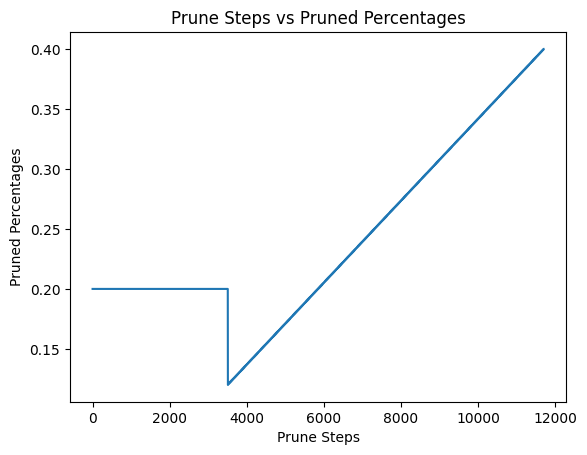
\includegraphics[width=0.6\textwidth]{output_prune_percentages.png}
    \caption{Prune percentages per batch}
    \label{fig:prune_percent}
\end{figure}

\subsection{Pruning Effectiveness}

The dynamic pruning strategy achieves an average pruning rate of 24.4\% across the training process, maintaining computational efficiency comparable to baseline approaches and introducing negligible overhead. Notably, the method achieves an optimal balance between accuracy and computational efficiency, outperforming static pruning in this regard.

\subsection{Comparative Analysis}\label{comparative_analysis}

\begin{figure}[h]
    \centering
    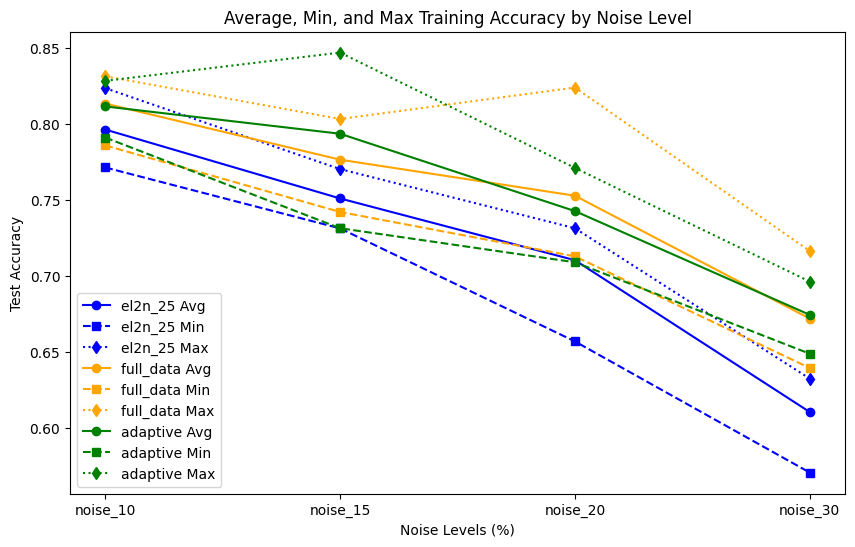
\includegraphics[width=0.8\textwidth]{output_comparison2.png}
    \caption{Comparison of training methods}
    \label{fig:comparison}
\end{figure}

Table~\ref{tab:results} summarizes the test accuracy across different noise levels, plotted in Figure \ref{fig:comparison}:

\begin{table}[h]
\caption{Test Accuracy (\%) at Different Noise Levels}
\label{tab:results}
\centering
\begin{tabular}{lccccc}
\toprule
Method & 10\% & 15\% & 20\% & 30\% \\
\midrule
Full Training & \textbf{81.33} & 77.64 & \textbf{75.27} & 67.18 \\
Static EL2N & 79.63 & 75.09 & 71.03 & 61.03 \\
Adaptive EL2N & 81.14 & \textbf{79.35} & 74.26 & \textbf{67.43} \\
\bottomrule
\end{tabular}
\end{table}

The empirical results underscore that the adaptive pruning approach achieves performance metrics closely aligned with those of full training, while consistently and significantly outperforming static pruning. These benefits persist across all evaluated noise levels, highlighting the robustness and adaptability of the proposed methodology. Furthermore, these gains are realized while training on a reduced dataset, illustrating the capability of dynamic pruning strategies to effectively manage noisy datasets without compromising model accuracy.

These findings support our hypothesis that dynamic adaptation of pruning strategies throughout training can effectively handle noisy datasets while maintaining model performance. The approach ensures not only high model performance but also computational efficiency, offering a compelling solution for real-world applications where noise is prevalent.

\section{Project Challenges}

Our research encountered several significant challenges that merit discussion. These challenges not only shaped our experimental approach but also highlight important considerations for future work in dynamic dataset pruning.

\subsection{Computational Resources and Time Constraints}

Training deep learning models with various noise levels and pruning strategies required substantial computational resources. Even with access to A100 GPUs, executing more than 24 experimental runs across a two-week period proved time-intensive. Each run needed to be carefully monitored and validated, limiting our ability to explore a broader range of hyperparameters and architectures.

\subsection{Hyperparameter Complexity}

The introduction of dynamic pruning added several new hyperparameters to an already complex training process, such as the initial pruning percentage, transition timing between pruning phases, rate of pruning adjustment and interaction with existing hyperparameters (learning rate, batch size).

The potential combinations grew exponentially, making exhaustive exploration impractical. The interaction between pruning strategies and traditional training parameters remains an open question.

\subsection{Evaluation}

Noisy datasets complicated the evaluation process by producing results with test accuracy exhibited non-monotonic behavior (e.g., better performance at 2K steps than at 4K steps with 20\% noise). Additionally, traditional metrics became less reliable as noise levels increased and distinguishing between pruning effects and noise effects becomes more challenging.

Our primary hypothesis, that dynamic tuning of pruning-related hyperparameters throughout training improves accuracy for noisy datasets, relied heavily on heuristics. This necessitated extensive empirical validation, which was constrained by the aforementioned computational limitations.

These challenges underscore the need for more efficient methods for hyperparameter optimization, better theoretical understanding of pruning dynamics, improved metrics for evaluating performance on noisy datasets, and standardized benchmarks for comparing dynamic pruning strategies.

Despite these challenges, our results demonstrate the potential of dynamic pruning strategies. Future work will need to address these limitations systematically, potentially through automated hyperparameter optimization and more sophisticated evaluation metrics.

\section{Future Work}

Our current results, while promising, suggest several compelling directions for future research. First, extending the experimental validation would strengthen our findings. This includes conducting additional runs to establish statistical significance and eliminate potential random effects in our current results. More comprehensive validation could also involve scaling to larger datasets such as CIFAR-100, which would help verify the approach's effectiveness on more complex classification tasks, and applying this algorithm to different model architectures. 

A particularly interesting direction involves extending our dynamic pruning framework beyond vision tasks. Specifically, adapting the method for different architectures like GPT and exploring its effectiveness on text, voice, and video data would demonstrate the framework's generalizability across domains. This cross-domain validation is especially important given the prevalence of noisy labels in real-world datasets across various modalities.

From an algorithmic perspective, several optimizations merit investigation. The current pruning percentage settings across different training phases, while effective, could benefit from more principled tuning approaches. We envision developing methods for automatic hyperparameter optimization specifically focused on the newly introduced parameters in our framework.

While we have focused primarily on improving training efficiency in the presence of noisy data, there are potentially important implications for bias reduction in machine learning models. Specifically, investigating how dynamic pruning affects representation of minority groups in the training data could yield insights into creating more equitable learning systems.

\section{Conclusion}
We presented a dynamic EL2N-based pruning approach that effectively handles noisy datasets while maintaining model performance. Our method demonstrates significant improvements over static pruning approaches, particularly in high-noise scenarios. The results suggest that adaptive pruning strategies can better capture the changing dynamics of model training, leading to more robust and efficient learning.

\begin{thebibliography}{9}

\bibitem{paul2021}
Paul et al., "Deep Learning on a Data Diet: Finding Important Examples Early in Training," \textit{arXiv:2107.07075}, 2021.

\bibitem{kirsch2023}
Kirsch, A., "Does 'Deep Learning on a Data Diet' reproduce?" \textit{OATML Technical Report}, 2023.

\bibitem{coleman2019}
Cody Coleman, Christopher Yeh, Stephen Mussmann, Baharan Mirzasoleiman, Peter Bailis, Percy Liang, Jure Leskovec, Matei Zaharia, "Selection via Proxy: Efficient Data Selection for Deep Learning," \textit{arXiv:1906.11829}, 2019.

\bibitem{mirzasoleiman2019}
Baharan Mirzasoleiman, Jeff Bilmes, Jure Leskovec, "Coresets for Data-efficient Training of Machine Learning Models," \textit{arXiv:1906.01827}, 2019.

\bibitem{mirzasoleiman2020}
Baharan Mirzasoleiman, Kaidi Cao, Jure Leskovec, "Coresets for Robust Training of Neural Networks against Noisy Labels," \textit{arXiv:2011.07451}, 2020.

\bibitem{bertsekas2015}
Bertsekas, D. P., "Incremental gradient, subgradient, and proximal methods for convex optimization: A survey," \textit{arXiv preprint arXiv:1507.01030}, 2015b.

\bibitem{glorot2010}
Glorot, X. and Bengio, Y., "Understanding the difficulty of training deep feedforward neural networks," in \textit{Proceedings of the Thirteenth International Conference on Artificial Intelligence and Statistics}, pp. 249–256, 2010.

\bibitem{kaufman1987}
Kaufman, L., Rousseeuw, P., and Dodge, Y., "Clustering by means of medoids in statistical data analysis," 1987.

\bibitem{lin2009}
Lin, H., Bilmes, J., and Xie, S., "Graph-based submodular selection for extractive summarization," in \textit{Proceedings of the IEEE Automatic Speech Recognition and Understanding (ASRU)}, Merano, Italy, December 2009.

\end{thebibliography}


\appendix
\section{Additional Material}

\begin{figure}[h]
    \centering
    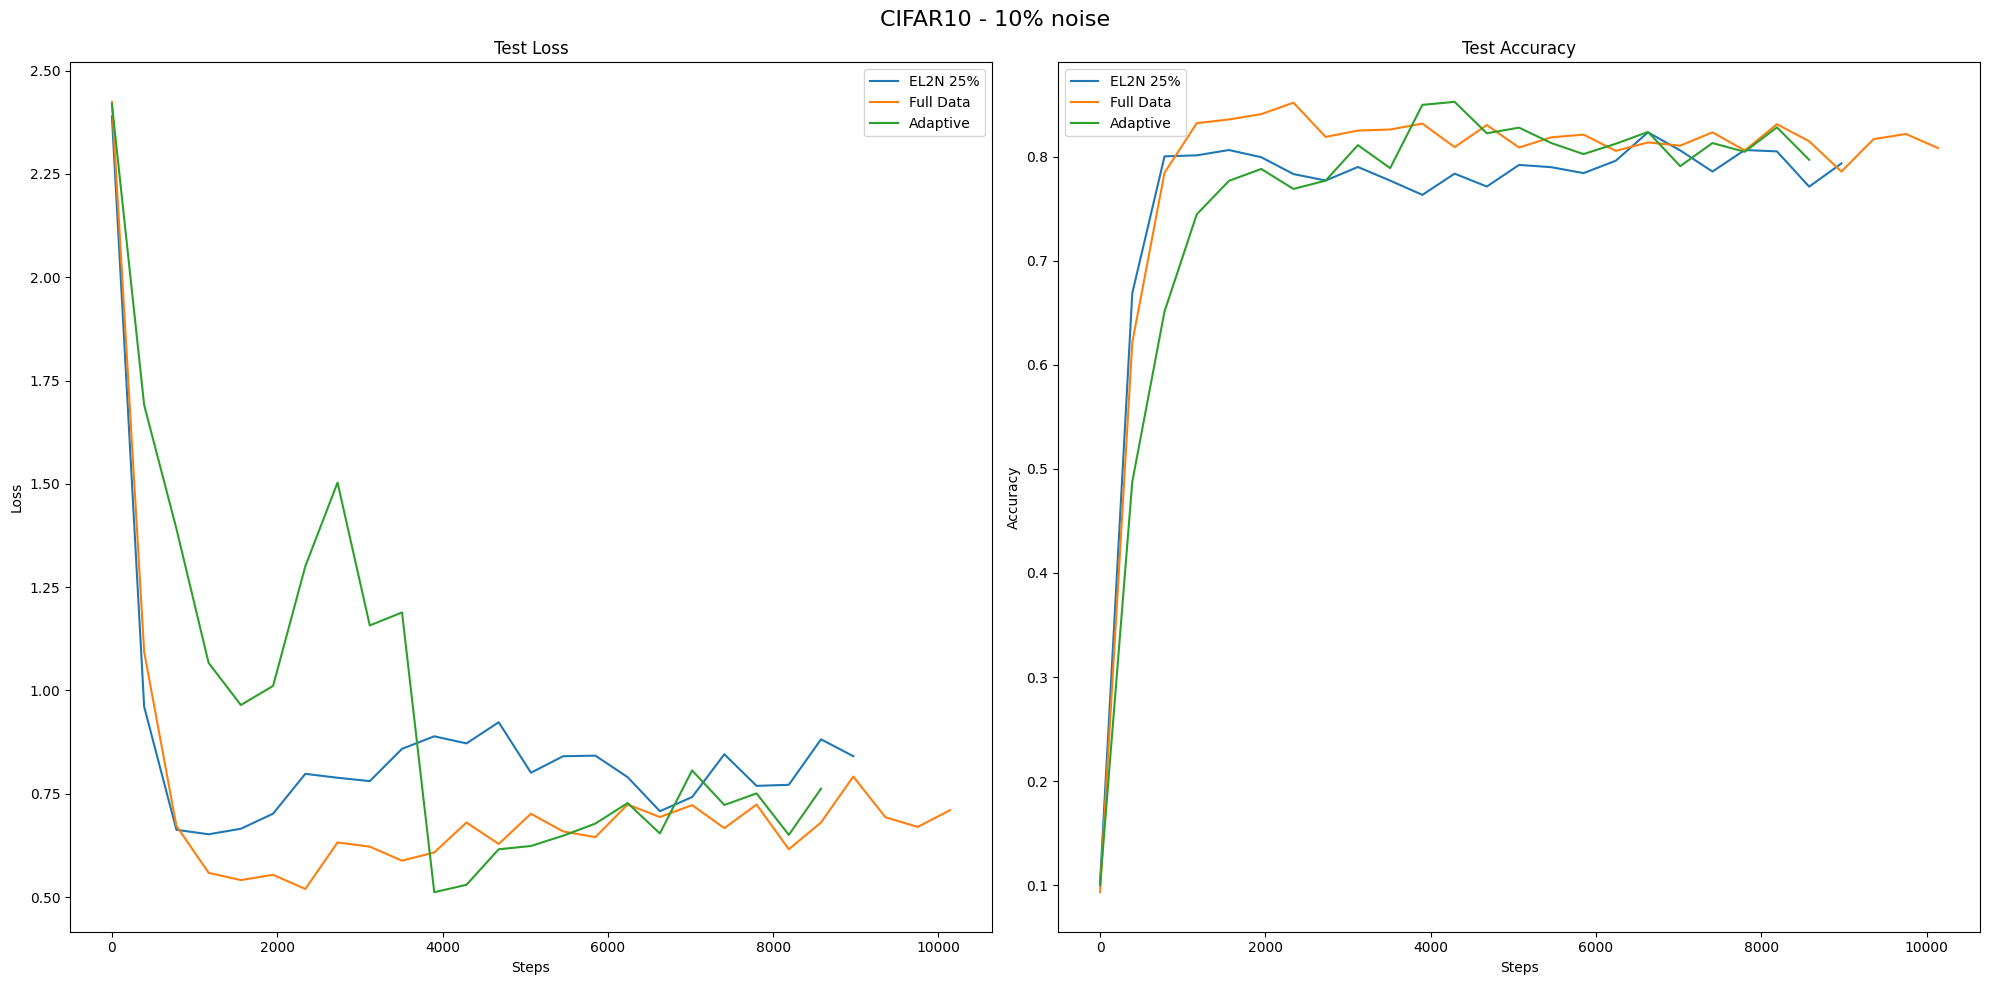
\includegraphics[width=1\textwidth]{output_noise_10.png}
    \caption{Test curves at 10\% noise}
    \label{fig:output_10}
\end{figure}

\begin{figure}[h]
    \centering
    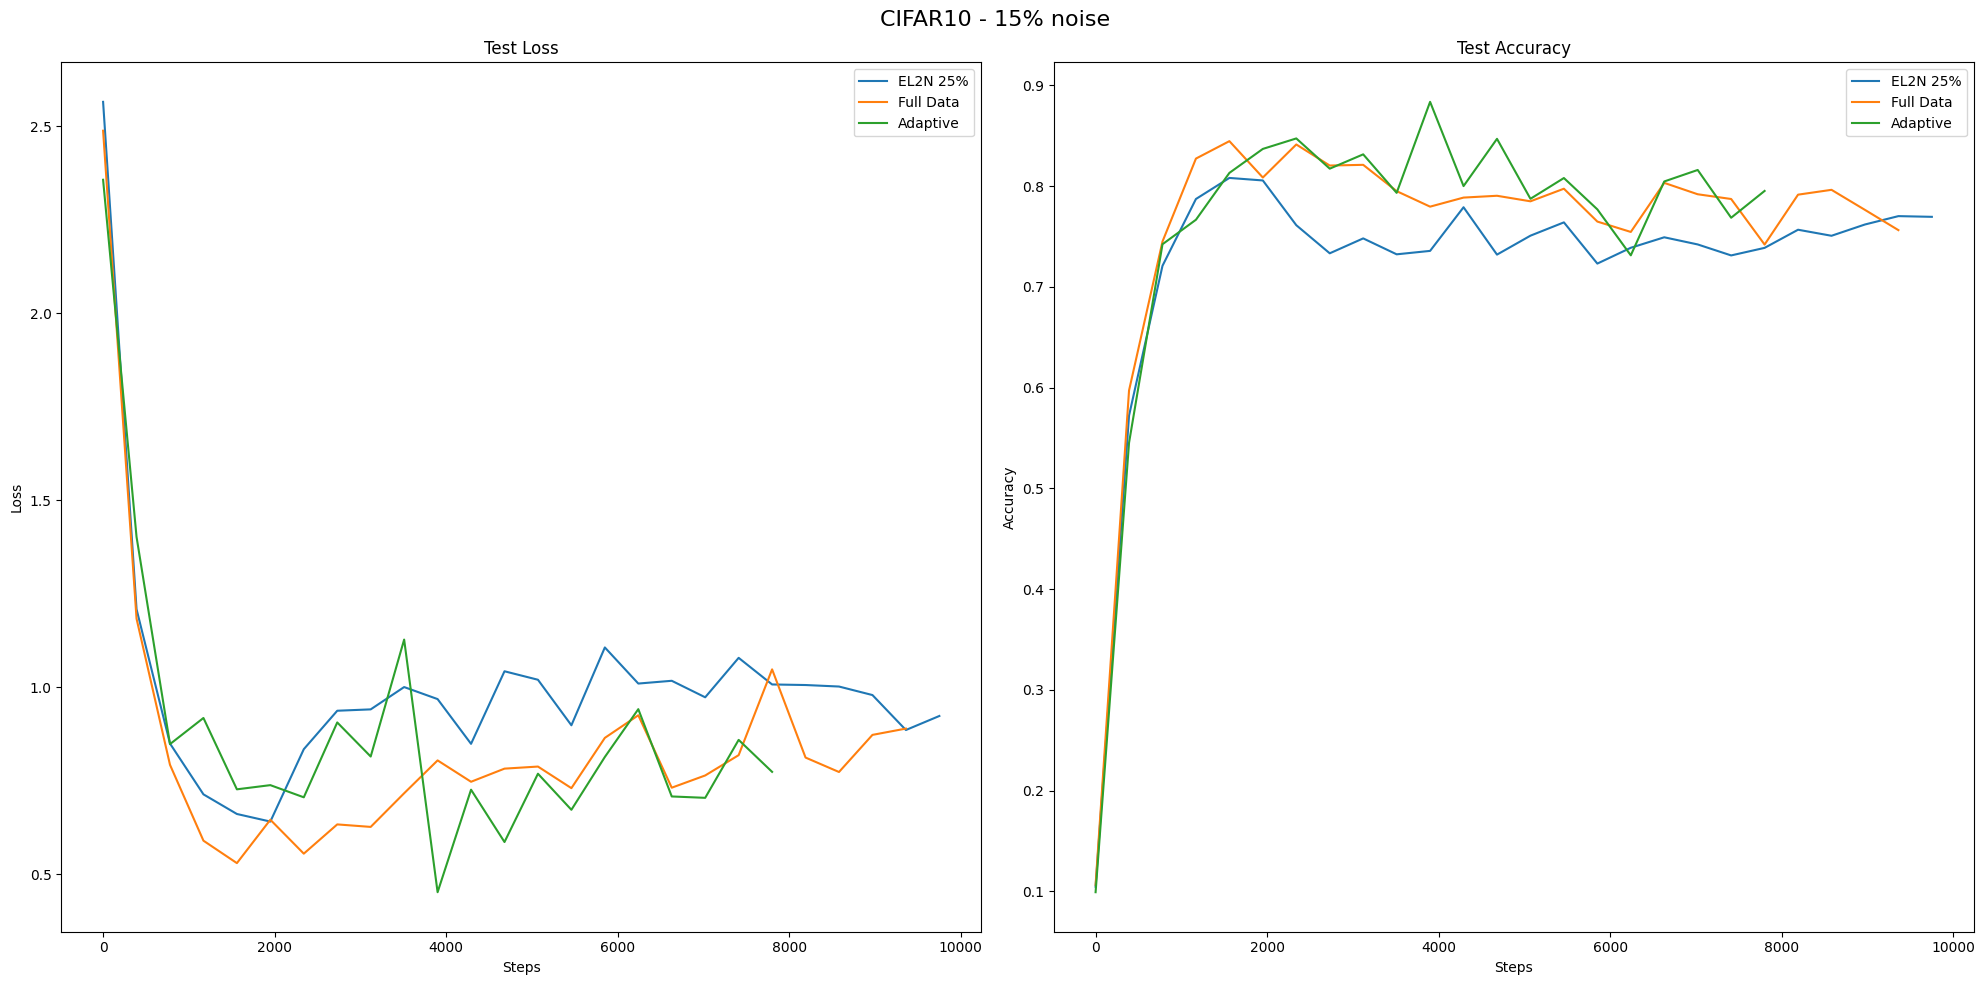
\includegraphics[width=1\textwidth]{output_noise_15.png}
    \caption{Test curves at 15\% noise}
    \label{fig:output_15}
\end{figure}

\begin{figure}[h]
    \centering
    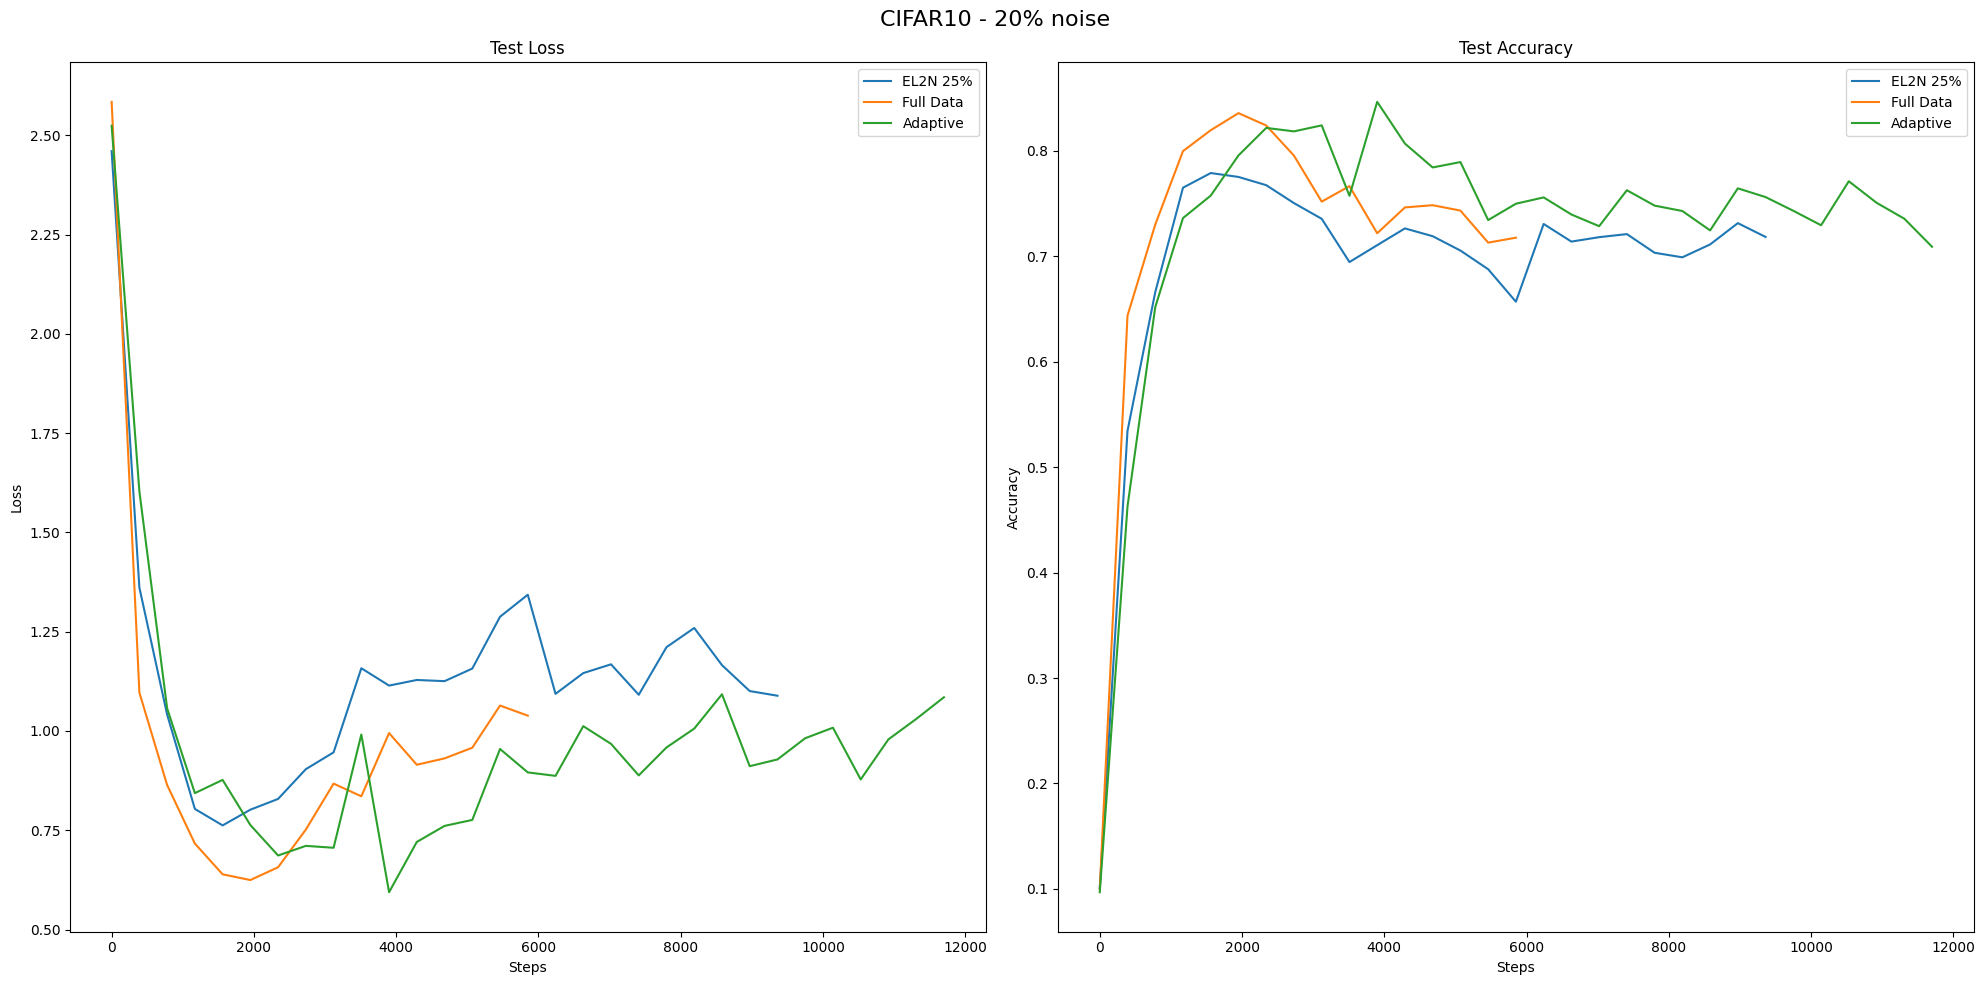
\includegraphics[width=1\textwidth]{output_noise_20.png}
    \caption{Test curves at 20\% noise}
    \label{fig:output_20}
\end{figure}

\begin{figure}[h]
    \centering
    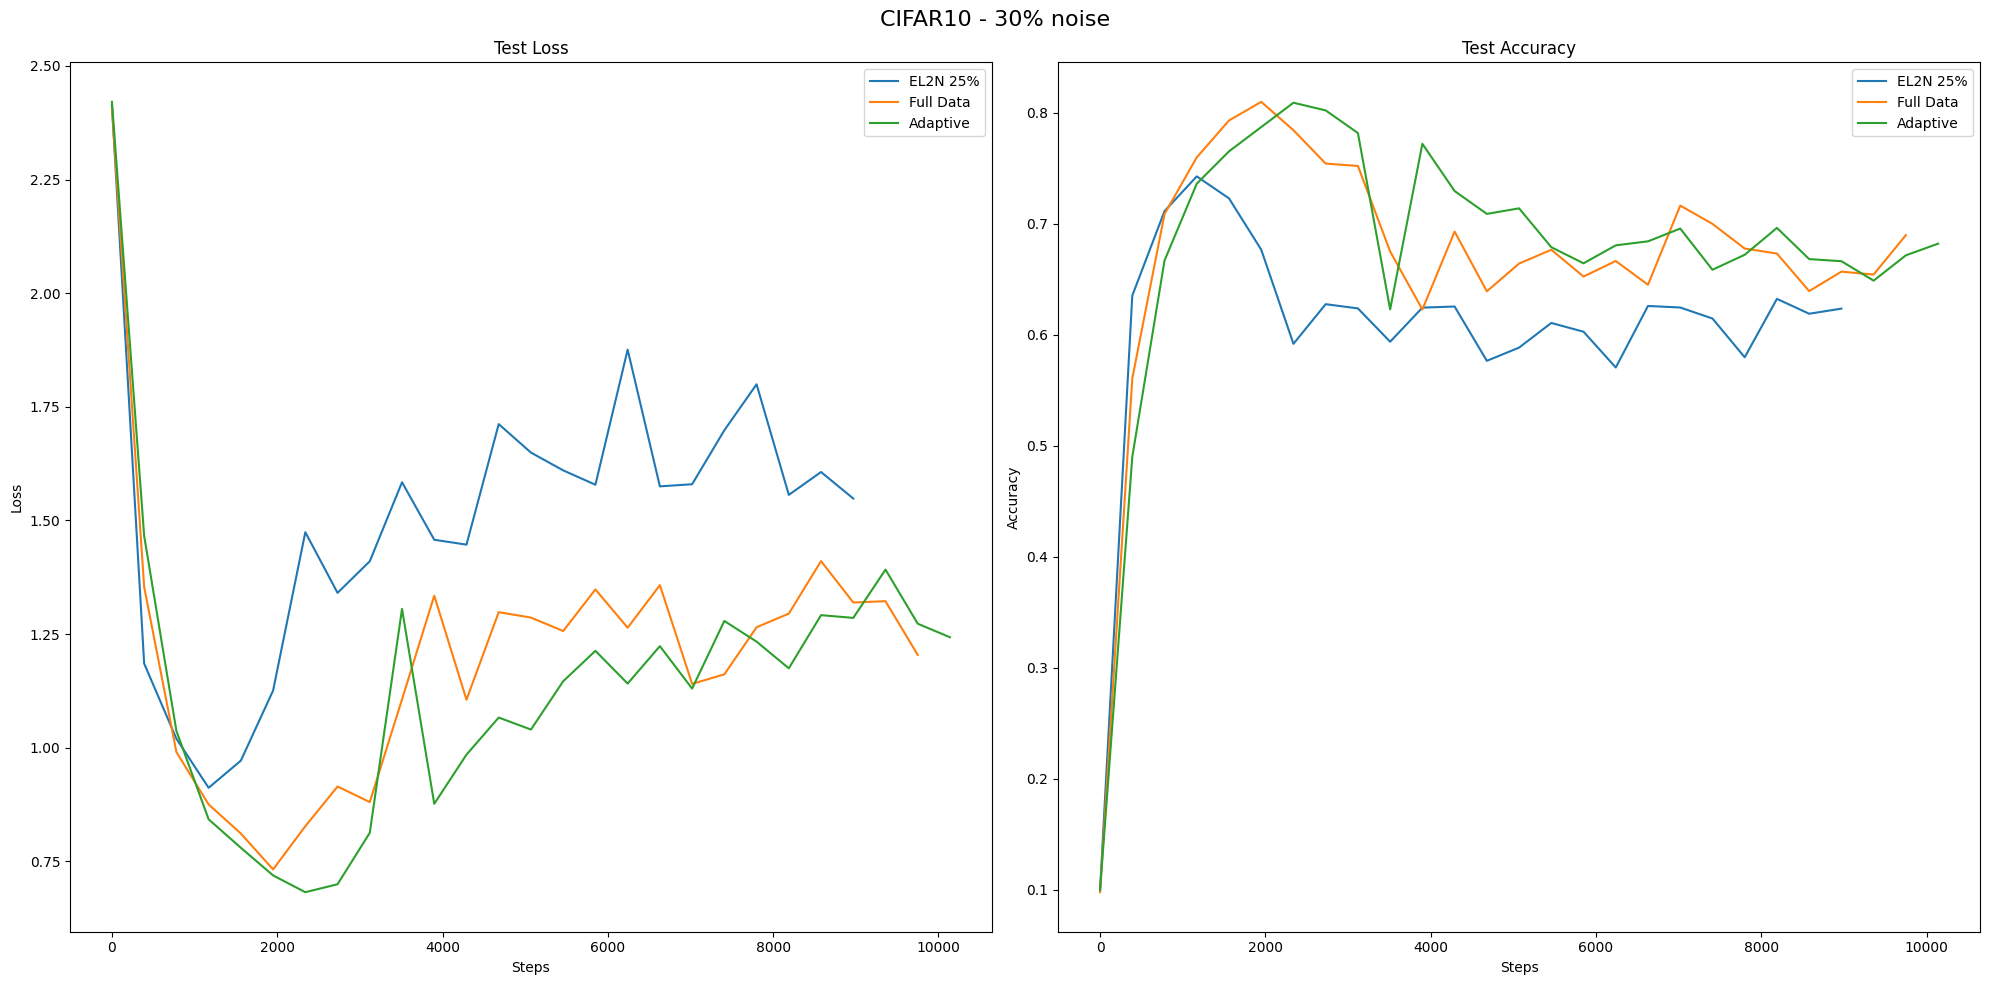
\includegraphics[width=1\textwidth]{output_noise_30.png}
    \caption{Test curves at 30\% noise}
    \label{fig:output_30}
\end{figure}

\end{document}
